              
\documentclass[12pt]{article}
 \usepackage[margin=1in]{geometry} 
\usepackage{amsmath,amsthm,amssymb,amsfonts, multirow, graphicx, float}
 
\newcommand{\N}{\mathbb{N}}
\newcommand{\Z}{\mathbb{Z}}
 
\newenvironment{problem}[2][Problem]{\begin{trivlist}
\item[\hskip \labelsep {\bfseries #1}\hskip \labelsep {\bfseries #2.}]}{\end{trivlist}}
%If you want to title your bold things something different just make another thing exactly like this but replace "problem" with the name of the thing you want, like theorem or lemma or whatever
 
\begin{document}
 
%\renewcommand{\qedsymbol}{\filledbox}
%Good resources for looking up how to do stuff:
%Binary operators: http://www.access2science.com/latex/Binary.html
%General help: http://en.wikibooks.org/wiki/LaTeX/Mathematics
%Or just google stuff
 
\title{Homework 2}
\author{Selma Wanna}
\maketitle
 
\begin{problem}{1}
Provide the DH Table and labeled figure of the RRP mechanism provided in Homework 2.
\end{problem}
 
 \begin{figure}[H]
     \centering
     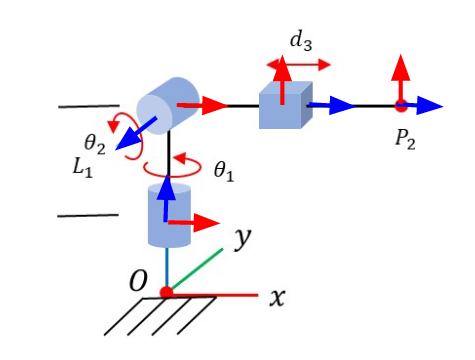
\includegraphics[width = 0.5\linewidth]{RRP.png}
     \caption{RRP mechanism labeled. The blue arrows represent the z axis for each frame. The red arrows represent the x axis for each frame.}
     \label{fig:rrp}
 \end{figure}


\begin{table}
\caption{RRP DH Parameters}
\begin{center}
\begin{tabular}{ c| c c c c }
 & $\theta$ & d & a & $\alpha$ \\ 
 \hline
 $A_1$ & $\theta_1$\textsuperscript{*} & 0 & 0 & $\frac{\pi}{2}$ \\  
 $A_2$ & $\theta_2$\textsuperscript{*} + $\frac{\pi}{2}$ & 0 & 0 & $\frac{\pi}{2}$ \\
 $A_3$ & 0 & $d_3$\textsuperscript{*} & 0 & 0
\end{tabular}
\end{center}
\end{table}





\pagebreak

\begin{problem}{2}
Provide the DH Table and labeled figure of the 7 DOF mechanism provided in Homework 2.
\end{problem}

 \begin{figure}[H]
     \centering
     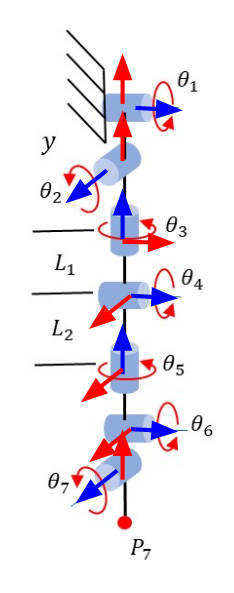
\includegraphics[width = 0.25\linewidth]{7dof.png}
     \caption{7 DOF mechanism labeled. The blue arrows represent the z axis for each frame. The red arrows represent the x axis for each frame.}
     \label{fig:7dof}
 \end{figure}

\begin{table}[H]
\caption{7DOF DH Parameters}
\begin{center}
\begin{tabular}{ c| c c c c }
 & $\theta$ & d & a & $\alpha$ \\ 
 \hline
 $A_1$ & $\theta_1$\textsuperscript{*} & 0 & 0 & -$\frac{\pi}{2}$ \\  
 $A_2$ & $\theta_2$\textsuperscript{*} - $\frac{\pi}{2}$ & 0 & 0 & -$\frac{\pi}{2}$ \\
 $A_3$ & $\theta_3$\textsuperscript{*} - $\frac{\pi}{2}$ & 0 & 0 & $\frac{\pi}{2}$ \\
 $A_4$ & $\theta_4$\textsuperscript{*} & $L_1$ & 0 & $\frac{\pi}{2}$ \\
 $A_4$ & $\theta_5$\textsuperscript{*} & $L_2$ & 0 & -$\frac{\pi}{2}$ \\
 $A_6$ & $\theta_6$\textsuperscript{*} - $\frac{\pi}{2}$ & 0 & 0 & -$\frac{\pi}{2}$ \\
 $A_7$ & $\theta_7$\textsuperscript{*} & 0 & 0 & 0
\end{tabular}
\end{center}
\end{table}
 
\end{document}
              